\chapter[SCP-039 长鼻工程师]{
    SCP-039 Proboscis Engineers\\
    SCP-039 长鼻工程师
}

\label{chap:SCP-039}

\begin{figure}[H]
    \centering
    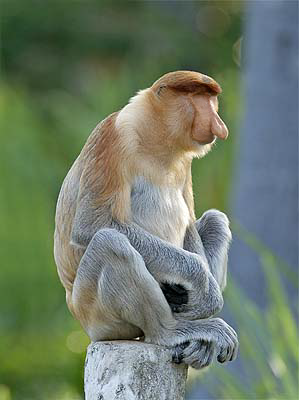
\includegraphics[width=0.5\linewidth]{images/SCP-039.png}
    \caption*{一只雄性SCP-039个体。}
\end{figure}

\bb{项目编号:}SCP-039

\bb{项目等级:}Euclid

\bb{特殊收容措施:}所有SCP-039个体应被收容于Site-77的\overtextnote{原生态观察室-2B(Wilderness Observation Chamber-2B)}中。应有至少两(2)名安保人员监控SCP-039房间内外,每六(6)小时换班。员工必须在站点安保的护卫之下进入SCP-039的房间,且只能为了进行研究或者每周一次的对房间内收容措施破坏和违禁物品的检查而进入。

SCP-039-8自20██年9月18日起怀孕;收容它的职责已移交给\overtextnote{兽医观察侧楼(veterinary observation wing)}的员工。

\bb{描述:}SCP-039是二十三(23)只在解剖学层面上发生了彻底变化的\ii{长鼻猴}(Nasalis larvatus)个体。SCP-039都没有眼睛和嘴,面部仅长有鼻子及附属的鼻道。SCP-039个体拥有灵敏的听觉和触觉,弥补了视觉的缺失。它们主要依靠身体接触来感知物体,以大声打响鼻作为回声定位的手段从而确定方位。尸检表明它们也没有消化系统;SCP-039个体如何获取营养——或者,反过来,它们在没有养分的情况下怎样生存——仍然是一项研究课题。

SCP-039个体显示出拥有智力的迹象,例如通过鼻子发声来交流、理解口头英语和对机械综合体的理解。成年个体已表现出操纵机械工具的能力,而且能够修理及制造多种技术设备,比如拆卸并重新组装内燃机、给公寓的一间小房间铺设电线等。测试表明,由于SCP-039个体经常互相转移注意力,SCP-039单独工作时效率比集体工作时更高。

在工作时,SCP-039个体偶尔会紧捂腹部,发出痛苦的声音。若附近放有食物,它们会将食物抹到脸上。有假设认为这表明SCP-039是普通\ii{长鼻猴}被人工改造后的产物,收容时回收的文件也支持该假设。(参见\bb{附录SCP-039-A})

SCP-039和\ii{长鼻猴}一样能够进行生殖和妊娠;该文档建立以来,已有五(5)只SCP-039个体诞生。SCP-039群体表现出了非常紧密的关系,新生儿常常由全部有能力的成年个体照料。新生个体具有与其它SCP-039个体相似的解剖学异常,但缺乏其它个体拥有的知识。父母会教给新生儿沟通方法和基本技巧,直到它们满六(6)个月,之后其它成年个体将传授技术本领。

SCP-039是从距离内华达州████████城区五十(50)公里的一个无人的研究所中回收的。收容过程中回收的文件指出该设施为██████ █████所有,该公司为提升人类天生能力的研究提供资金。二十(20)个SCP-039个体住在此地并维护研究所,居住时间长度未知。回收的其它文件表明曾有过一个意在提高人类智能的项目。该项目似乎在公司倒闭前不久被取消,后来公司资产被卖给一不知名组织。对██████ █████和接收其资产的组织的进一步调查尚未得到重要信息。

\bb{附录SCP-039-A} 在最初的收容过程中被回收的数份文件似乎注解了SCP-039开发过程中的初期原型阶段。研究已经开始以重现制造SCP-039新个体的过程;然而,收容之前笔记积累的损伤已使得不少部分无法辨认。

\begin{center}

\tred{打开文件SCP-039-1至16}

\tred{- 点击隐藏}

\end{center}

\begin{scpbox}

……移除后,它们的效率几乎翻了一倍,这还没算上休息和放假减少后多出来的时间。鉴于此次成功,我们正在考虑去掉身体上的其它孔洞,如果替换或者缺少这些部分不使产量下降的话。

Wernher今天看它们工作时注意到其中几只捂着肚子。好像它们产生了饿得肚子疼的幻觉,尽管它们已经不用吃东西了。不管它,除非影响到生产率。

\end{scpbox}

\begin{scpbox}

我们试着去掉眼部器官,让它们只凭记忆工作。几次无果而终的试验之后,我们竟然得到了一只得分和对照组测试几乎一样高的样本。我们决定按这个新方案做下去,如果成功就应用到所有样本身上。

\ii{编辑:}这一条的更新。去掉视觉后大多数样本的触觉灵敏度好像都增强了,而且引人注目的是,这让初次测试的对象们的生产率提高到了超出预期的水平。因此,我们将对所有可用的样本应用此项改变。其中几只不太适应,但是他们还是很擅长处理零配件。与此同时,我们已经把它们收入库存了。

\end{scpbox}

\begin{scpbox}

眼睛那件事成功之后,Damien建议我们增强听觉灵敏度来提高生产率。只要它们呆在工厂里就没啥问题,这儿没什么伤耳朵的东西。大概一周后开始测试。

\end{scpbox}

\begin{scpbox}

太成功了!在去掉了视力和对食物的需求,增强了听觉和触觉之后,我们得到了比最早的实验对象高出211\%的总增长。管理层已经决定给我们部门额外的时间来完成这个项目。再想想当时这个项目是当做玩笑卖给我们的!天哪,我感觉像在天上跳舞。

\ii{编辑:}今天出了点小事故。一个样本逃出了牢房,还拿走了几件工具。我们把它关了回去,重新封上了牢房。Alan说他明天会再把门检查一次。

\end{scpbox}
